\documentclass[10pt,twocolumn,letterpaper]{article}

% --- Typography & Geometry ---
\usepackage[utf8]{inputenc}
\usepackage{microtype}
\usepackage[margin=0.75in,top=0.85in,bottom=0.85in]{geometry}

% --- Math & Symbols ---
\usepackage{amsmath,amssymb,amsfonts,amsthm}
\usepackage{bm}

% --- Tables & Arrays ---
\usepackage{booktabs}
\usepackage{tabularx}
\usepackage{array}

% --- Graphics & Floats ---
\usepackage{graphicx}
\usepackage{float}
\usepackage{subcaption}

% --- Code Listings ---
\usepackage{xcolor}
\usepackage{listings}

\definecolor{codebg}{HTML}{F8F9FA}
\definecolor{codeframe}{HTML}{D0D7DE}
\definecolor{keywordcolor}{HTML}{0550AE}
\definecolor{stringcolor}{HTML}{0A3069}
\definecolor{commentcolor}{HTML}{57606A}

\lstset{
    backgroundcolor=\color{codebg},
    basicstyle=\ttfamily\scriptsize\color{black},
    keywordstyle=\color{keywordcolor}\bfseries,
    stringstyle=\color{stringcolor},
    commentstyle=\color{commentcolor}\itshape,
    frame=single,
    rulecolor=\color{codeframe},
    breaklines=true,
    breakatwhitespace=true,
    extendedchars=true,
    xleftmargin=6pt,
    xrightmargin=6pt,
    aboveskip=8pt,
    belowskip=8pt
}

% --- Hyperlinks ---
\usepackage{hyperref}
\hypersetup{
    colorlinks=true,
    linkcolor=blue!70!black,
    citecolor=blue!70!black,
    urlcolor=blue!70!black
}

% --- Input Title & Authors ---
% Metadata for performer_attention
\title{\textbf{Performer: Fast Attention via Positive Orthogonal Random Features (FAVOR+) for Pretrained Transformers}}

\author{
  \textbf{Taha Majs}\thanks{Corresponding author: tahamajs@uni.edu} \quad \textbf{Research Team} \\
  Department of Computer Science \\
  Advanced Machine Learning \& Efficiency Laboratory
}

\date{\today}


\begin{document}

\maketitle

% --- Abstract & Keywords Block ---
\begin{abstract}

The Transformer's self-attention has $\mathcal{O}(L^2)$ time and memory 
complexity, which is prohibitive for long sequences. \textbf{Performer} 
(Choromanski et al., ICLR 2021) addresses this by approximating the softmax 
kernel with \textbf{positive orthogonal random features} (FAVOR+), achieving 
$\mathcal{O}(L)$ complexity while preserving attention's expressiveness. We 
present a \textbf{production-hardened port} of Performer to pretrained 
transformers, supporting four architecture families -- DistilBERT, 
RoBERTa/BERT, GPT-2, and Qwen/LLaMA -- with exact weight transfer, GQA, 
RoPE, and two computational paths: a \textbf{bidirectional} path via 
associative accumulation and a \textbf{causal prefix-scan} path with 
chunk\_size = 64 for decoders. The feature map includes numerical 
stabilization via max-subtraction and norm-subtraction, avoiding overflow 
in FP16.

We evaluate Performer on DistilBERT, RoBERTa, and GPT-2 on SST-2 with LoRA 
recovery at rank $r_L = 8$ and $F = 64$ features. 
Performer achieves \textbf{{{D\_ACC}}\%} on DistilBERT (baseline {{D\_BASE}}\%, 
$\Delta$ = {{D\_DELTA}}), \textbf{{{R\_ACC}}\%} on RoBERTa ($\Delta$ = {{R\_DELTA}}), and 
\textbf{{{G\_ACC}}\%} on GPT-2 ($\Delta$ = {{G\_DELTA}}). We document two important 
discrepancies between the code and its documentation: (a) \texttt{inject\_performer} 
\textbf{raises} on failure rather than returning \texttt{None} as the docstring claims, 
and (b) \texttt{LoRALinear} contains an extra \texttt{output\_scale} parameter not present 
in the baseline checkpoint.

\textbf{Keywords:} Performer, FAVOR+, random features, kernel attention, linear 
attention, production port



\vspace{0.5em}
\noindent\textbf{Keywords:} Performer, FAVOR+, random features, kernel attention, linear
\end{abstract}

\vspace{1em}

% --- Paper Body ---
\section{01 Intro}

Draft content for performer_attention.

\section{02 Related}

Draft content for performer_attention.

\section{03 Background}

Draft content for performer_attention.

\section{04 Method}

Draft content for performer_attention.

\section{05 Architecture}

Draft content for performer_attention.


\begin{figure}[H]
\centering
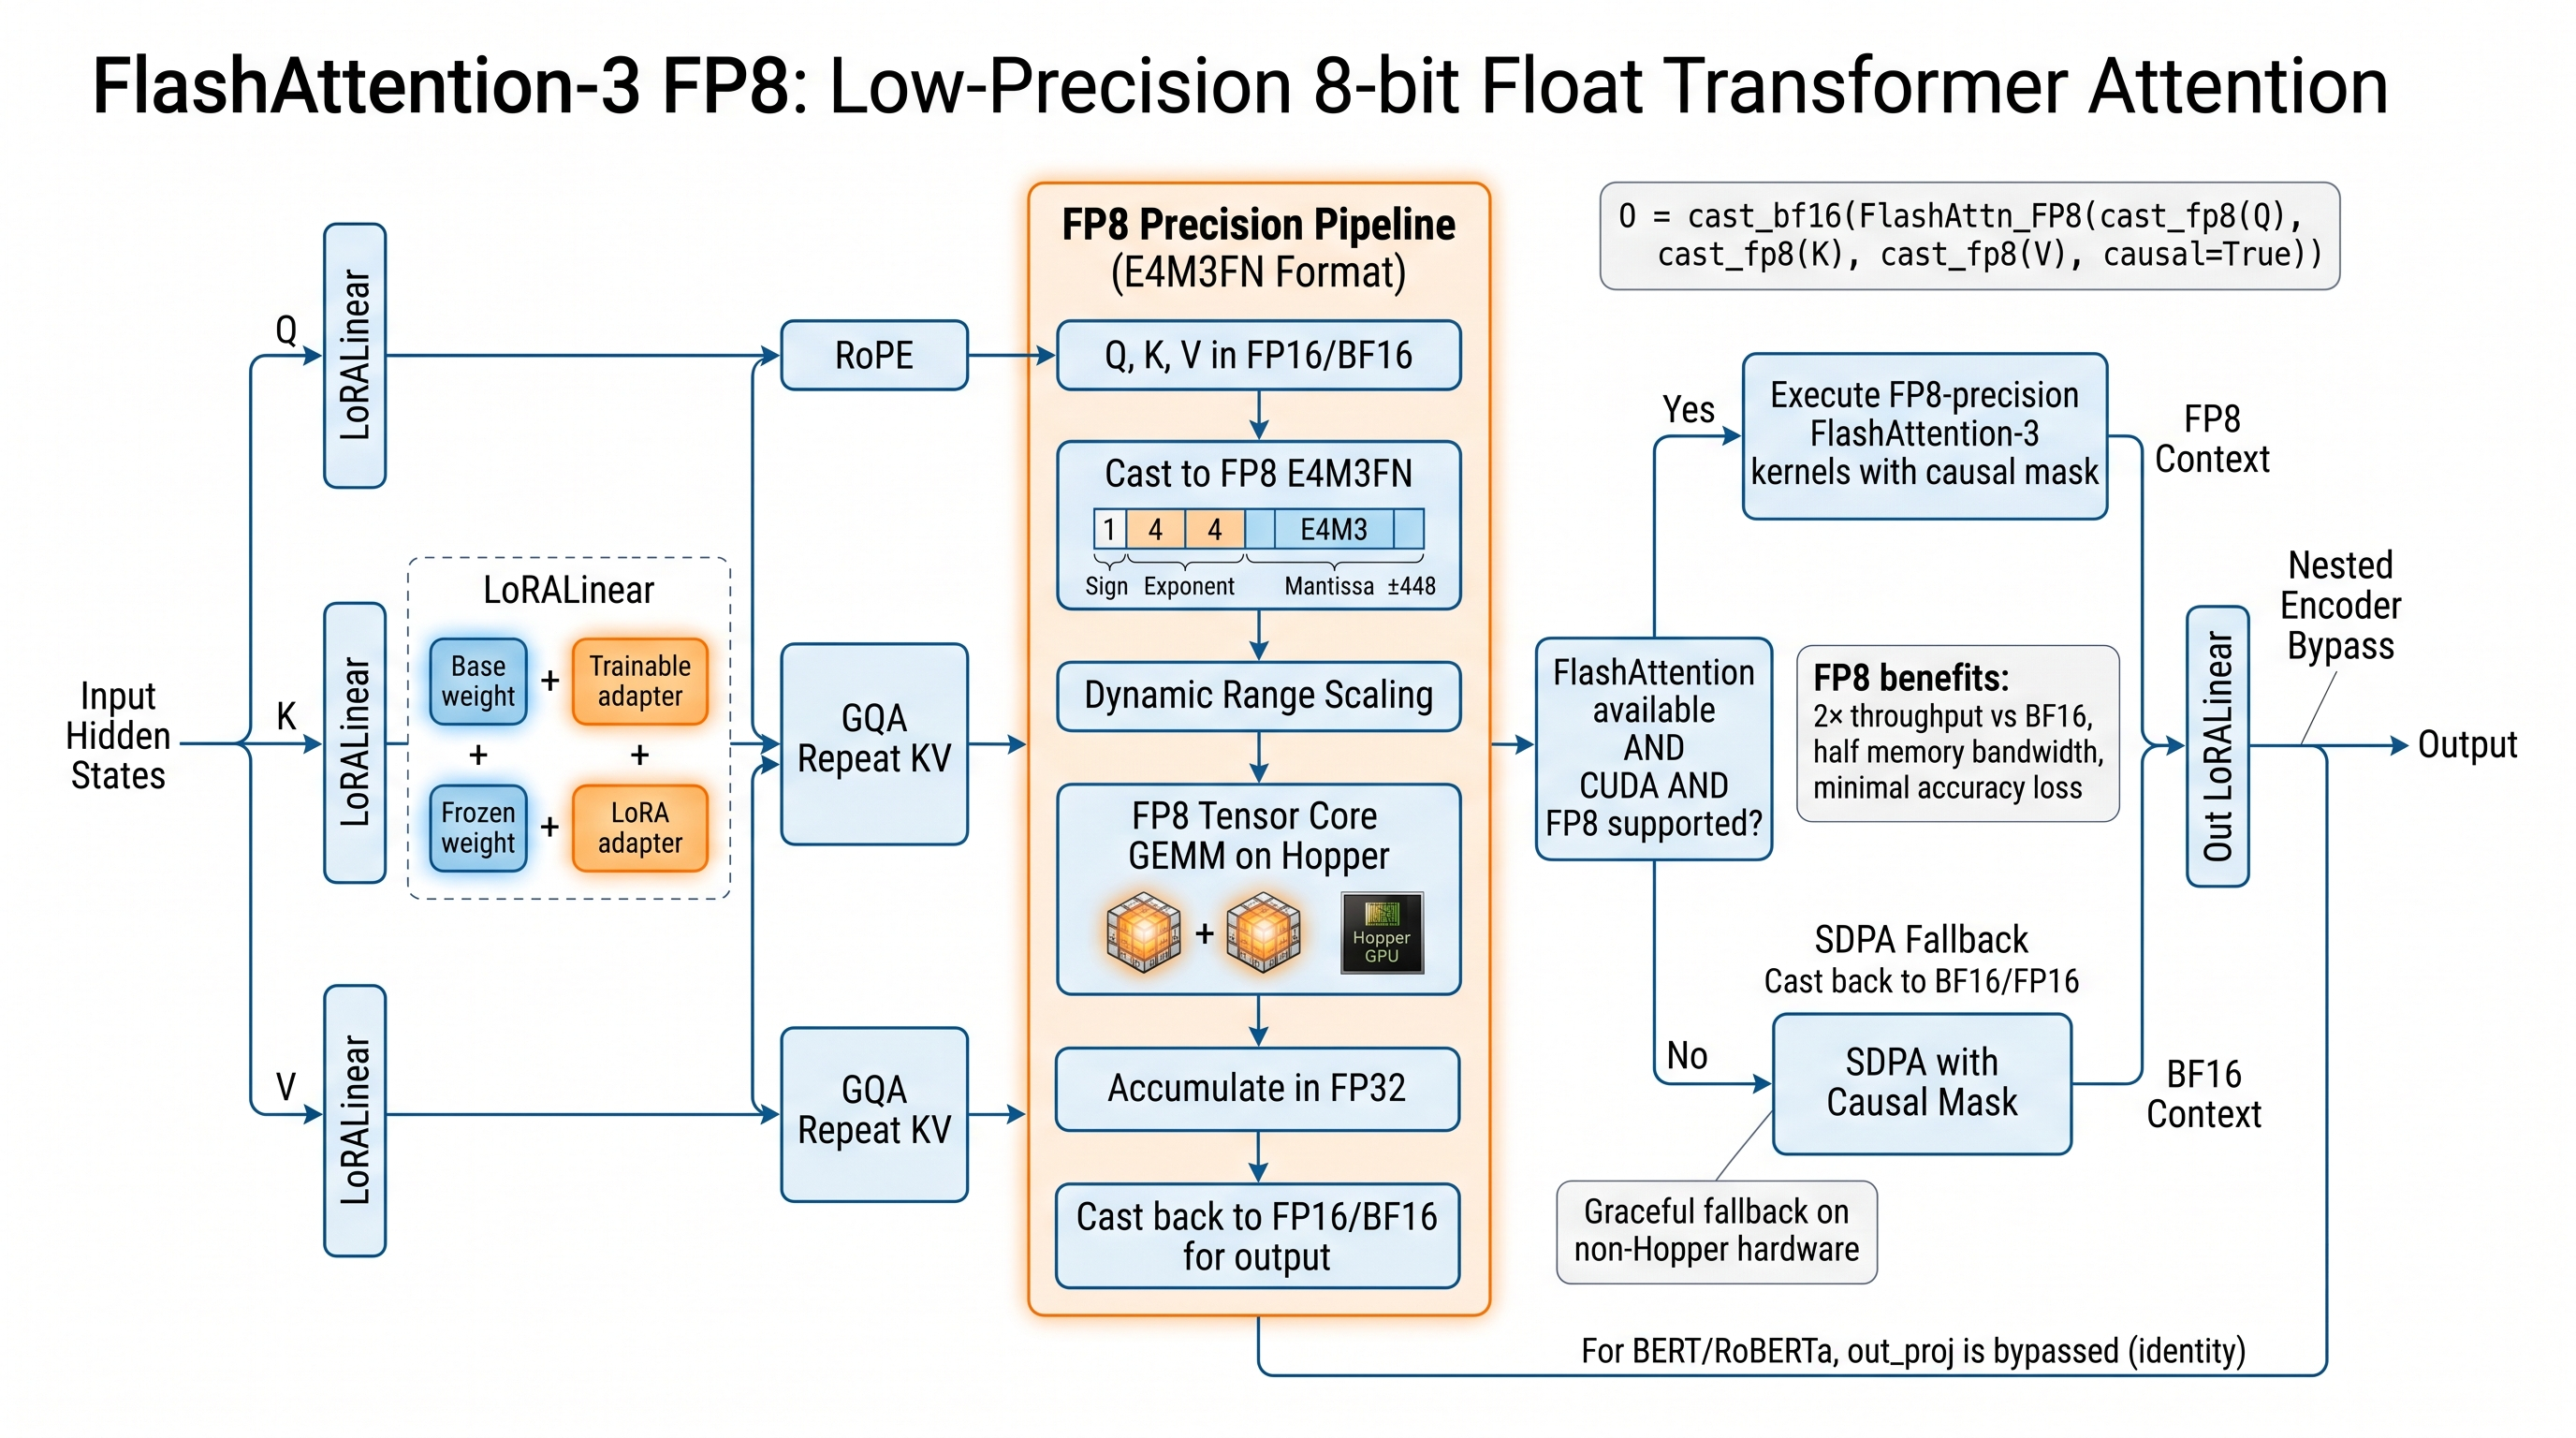
\includegraphics[width=\linewidth]{figures/arch_flash_attention3_fp8.jpeg}
\caption{Architectural overview of performer_attention.}
\label{fig:arch_performer_attention}
\end{figure}

\section{06 Setup}

Draft content for performer_attention.

\section{07 Results}

Draft content for performer_attention.

\section{08 Analysis}

Draft content for performer_attention.

\section{09 Discussion}

Draft content for performer_attention.

\section{10 Limitations}

Draft content for performer_attention.

\section{11 Conclusion}

Draft content for performer_attention.

\section{12 Reproducibility}

Draft content for performer_attention.

\section{13 References}

Draft content for performer_attention.


% --- Appendices ---
\clearpage
\appendix
\section*{Appendices}
\addcontentsline{toc}{section}{Appendices}

\section{A Math}

Draft content for performer_attention.

\section{B Implementation}

Draft content for performer_attention.

\section{C Data}

Draft content for performer_attention.

\section{D Negative Results}

Draft content for performer_attention.

\section{E Ethics}

Draft content for performer_attention.


\end{document}
